\section{Conditional Identity and Approximation Limits}
\label{app:proof}
Write $F\setminus P=G\cup B$, where $B$ is either $\varnothing$ or $\{b\}$,
independently of $G$. Then
$J_p(P)=(1-p)\E R(G)+p\E R(G\cup\{b\})$, while
$J_p(P\cup\{b\})=\E R(G)$. Subtraction proves Eq.~\eqref{eq:benefit} without
smoothness or additive-loss assumptions. Setting all outside probabilities to
zero reduces $V_b$ to $I_b$; this special case is not the general multi-fault
objective. Exact enumeration of the eight states in Section~\ref{sec:limits}
gives $J_p(\{a\})-J_p(\{b\})=p(p-.1)$, proving the counterexample.

For an equal-budget exchange, let $a\in P$, $b\notin P$ and
$P'=P\setminus\{a\}\cup\{b\}$. Sample $G$ over all other unprotected coordinates,
excluding $a,b$. The exact identity is
\begin{equation}
J_p(P')-J_p(P)=p\E_G[R(G\cup\{a\})-R(G\cup\{b\})].
\end{equation}
A deterministic path of legal exchanges can compare frozen masks. Contributions
along a path share a master field and are summed before computing uncertainty;
path steps are not independent replications. The identity applies to complete-file
ROC-AUC risk because it only requires a scalar response. It does not require, or
permit substituting, an additive per-window loss.

If an approximate risk table is uniformly within $\epsilon$ of the exact table
over the admissible masks, its minimizing mask has regret at most $2\epsilon$:
compare approximate and exact risks at the approximate and exact minimizers,
and use the approximate minimizer's inequality between them. This elementary
bound distinguishes numerical approximation error from Monte Carlo selection
error. A sum of absolute omitted interaction terms can upper-bound a polynomial
remainder, but at large candidate dimension such worst-case bounds can be
vacuous. Bounded numerical checks do not establish scalable selection benefit.
The Boolean/multilinear foundations are standard~\cite{odonnell2014analysis};
we do not present an unexecuted spectral program as an empirical contribution.

\section{Auxiliary Losses and Reproducibility}
\begin{figure}[p]\centering
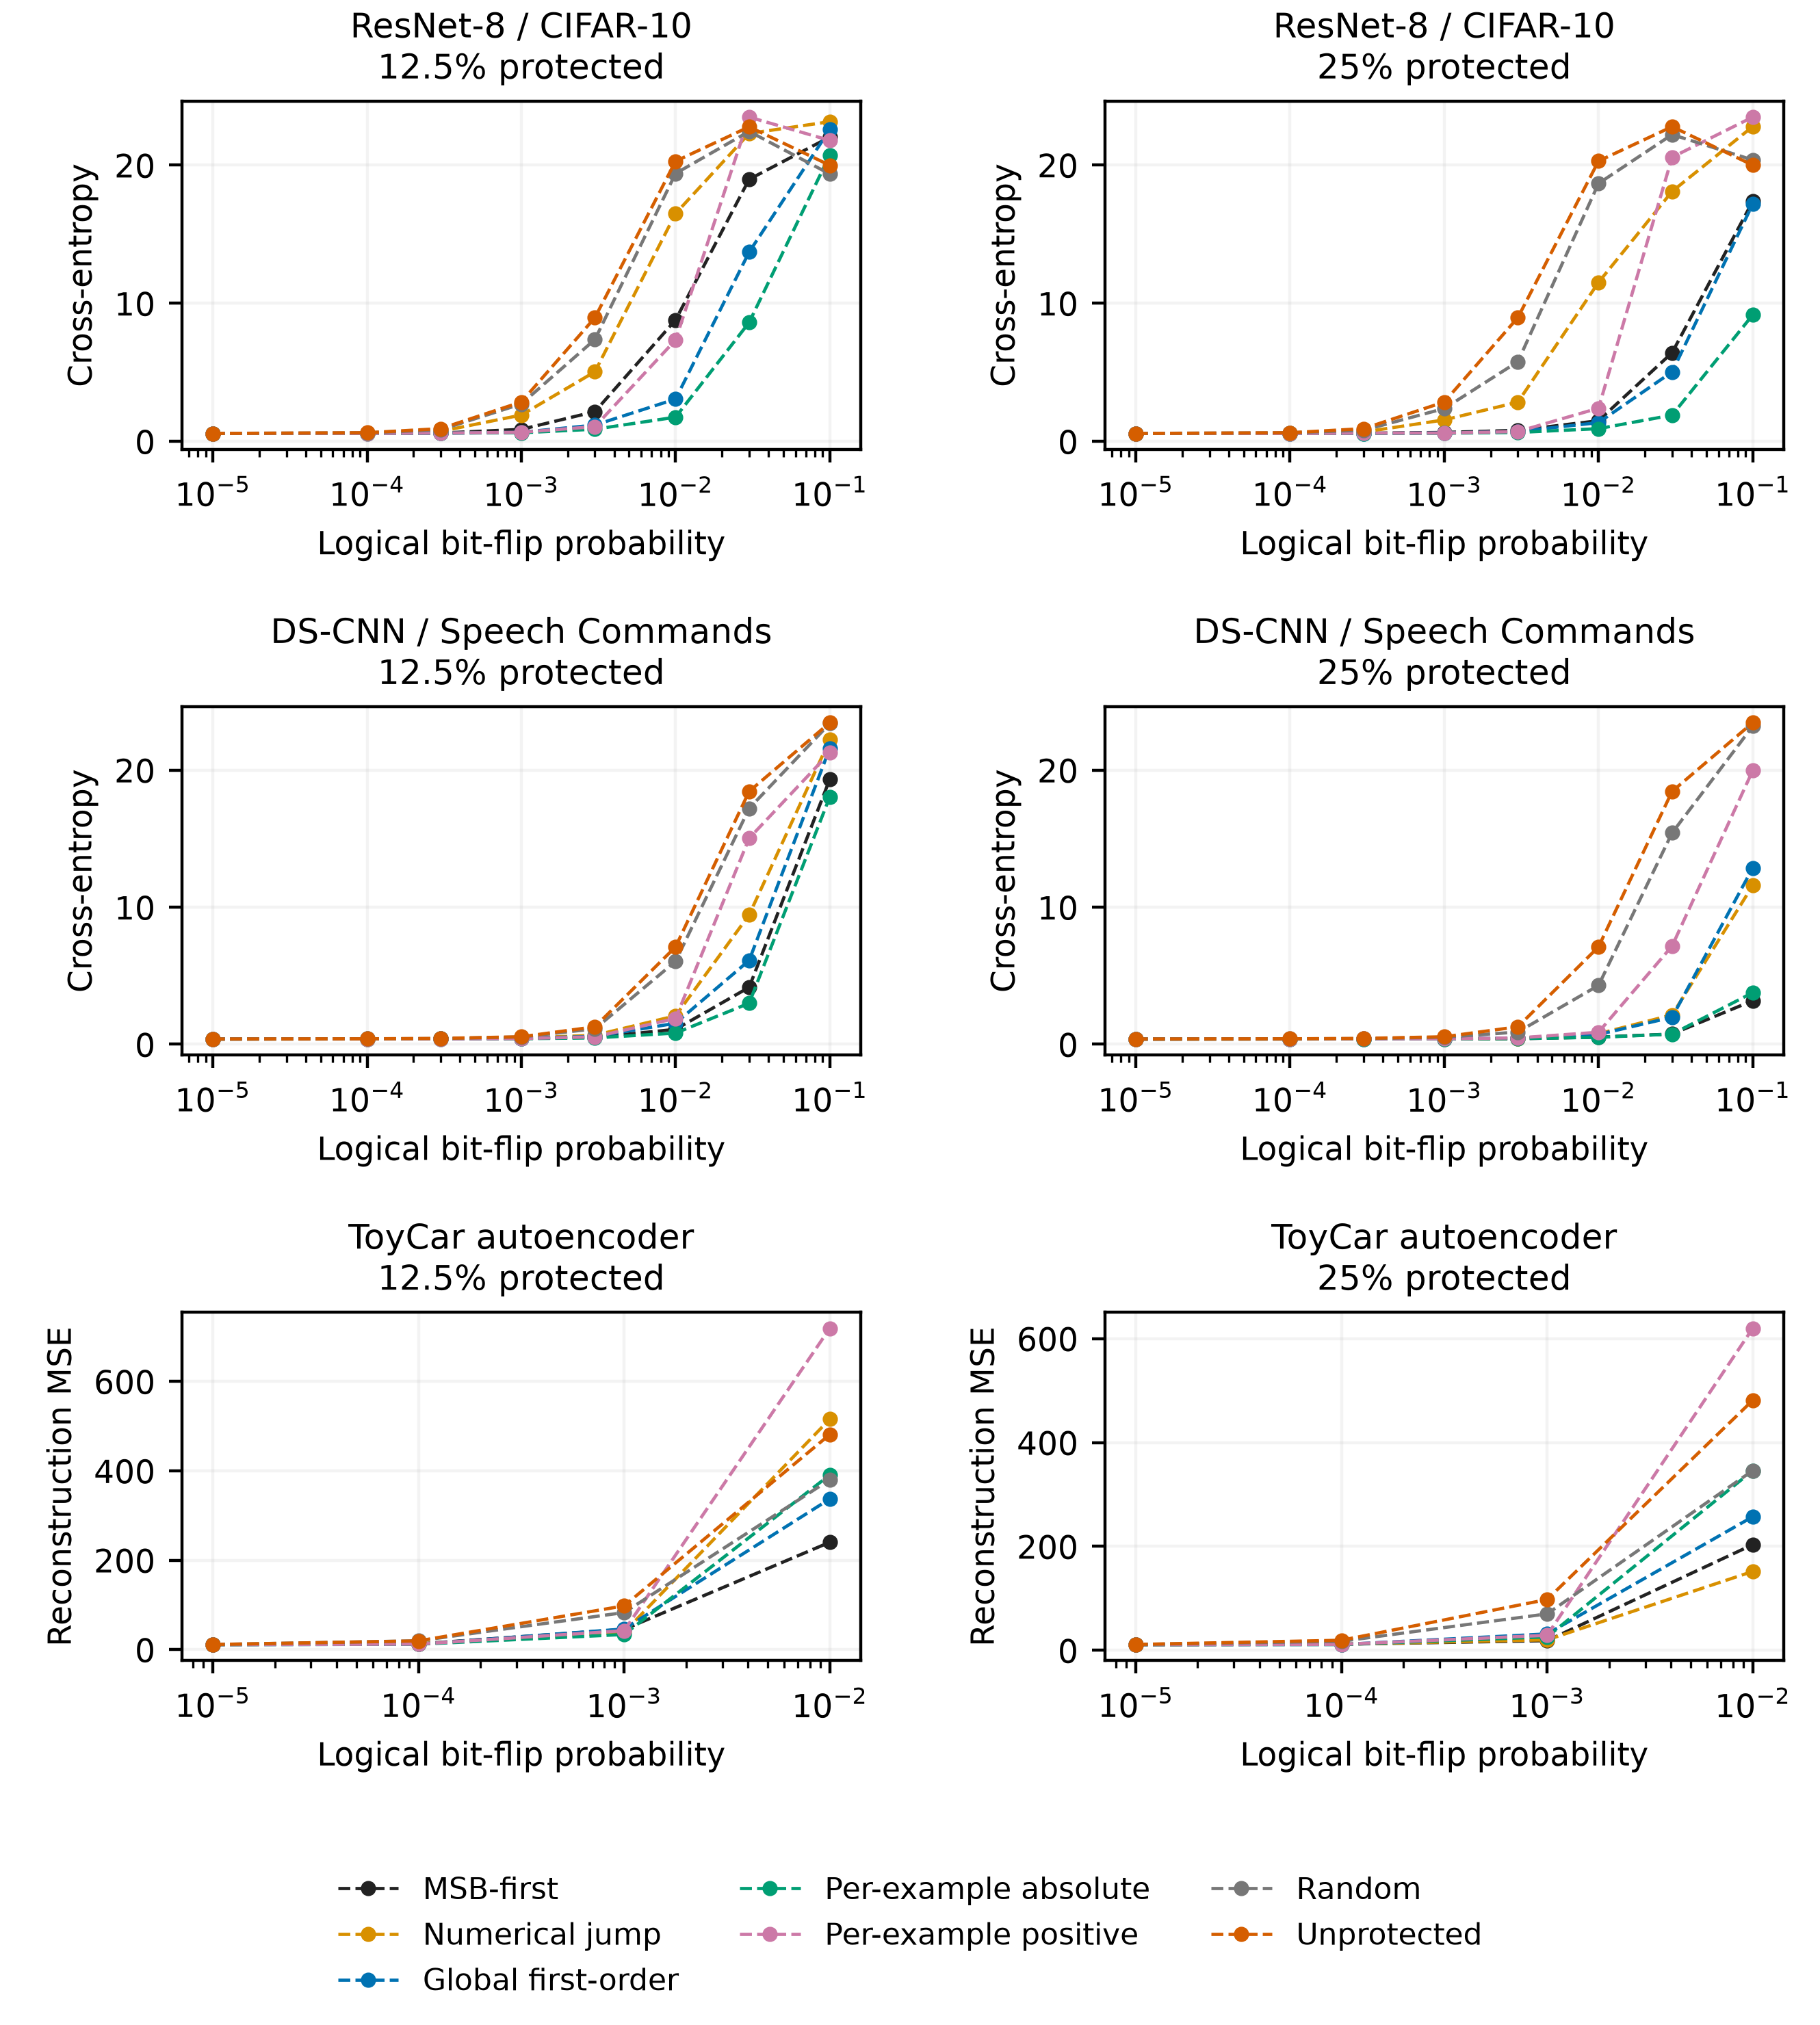
\includegraphics[width=.98\linewidth]{loss_ber.png}
\caption{\textbf{Does the auxiliary loss tell the same story as task quality?} Mean exact reference cross-entropy for the two classifiers and reconstruction MSE for ToyCar across all measured BERs. Units remain separate; no cross-task averaging is performed. The companion loss is used only for ranking. These curves show means; the accompanying numerical supplement retains per-condition standard deviations, standard errors through sample counts, and field-$t$ intervals. In particular, reduced ToyCar MSE need not improve file ROC-AUC.}
\Description{Six auxiliary-loss panels retain all six policies and unprotected controls. ToyCar reconstruction-error trends differ from its file-level AUC trends.}
\label{fig:loss}\end{figure}

The supplementary evidence package contains exact checkpoint and sample
identities, source payload and artifact hashes, raw-derived condition tables,
paired comparisons, figure/table recipes, and the archived method definitions.
Publication figures are generated only from verified finalized measurements.
The audit rechecked 126 finalized records and 612 consumed files, recomputed
10,112 static trial rows into 358 condition summaries, and checked 2,184 paired
summary means and intervals. This scope does not assert that every unused file
in every historical directory was rehashed. Exact masks were hash-verified;
their large files were not re-enumerated during manuscript assembly.

Candidate correlations, pool-level intervals and field-level intervals retain
different sampling units. Ranking masks remain tied to their own construction
seeds. The frozen checkpoints are not retrained for a presentation change.
Original bundles are unchanged, and supplementary figures and tables do not
constitute new scientific trials. The build instructions separate offline
evidence processing from model execution and give the pinned source/backend
requirements for locating the original runs.
